\chapter{拘束系とハミルトン運動}

\lectureoverview{二つの拘束系は、ラグランジュ力学がなぜこれほど有効であるかを示している。適切な座標を選んでしまえば、運動方程式とその保存則は、拘束力を陽に計算することなく導かれる。同じ例はさらにハミルトン力学へと導く。そこでは座標と運動量が位相空間をなし、調和振動子は剛体回転となり、ハミルトンの二つの一階方程式が各々の二階のオイラー--ラグランジュ方程式に取って代わる。}

\section{力学の問題を解くとはどういうことか}

ラグランジュの方法の直接の目的は実用的である。床の上を滑るくさびと二重振り子はどちらもニュートンの法則で扱えるが、未知の接触力と張力のため、計算の整理はたちまち厄介になる。ラグランジュ力学の規則をひとたび知れば、同じ問題は統制された手順の列となる。
\begin{enumerate}
  \item 瞬間的な配置を指定する独立な座標を選ぶ。
  \item それらの座標で運動エネルギーと位置エネルギーを表す。
  \item \(L=T-V\) を作り、オイラー--ラグランジュ方程式を適用する。
\end{enumerate}

当面の目的にとっては、運動方程式が正しく書き下された時点で、その問題はすでに\emph{解けた}のである。閉じた形の軌道がなお欲しいこともあるが、それは別の問題である。非線形微分方程式は、力学的な設定が完了しさえすれば数値的に積分できる。難しい部分はしばしば積分ではなく、余分な未知の力を導入することなく拘束を取り込む変数を見つけることにある。

\section{動くくさびの上を滑る質点}

質量 \(M\) のくさびが、水平面に沿って摩擦なく滑るように拘束されている場合を考える。質量 \(m\) の点状の質点は、傾斜面の上にとどまるように拘束されている。自由度は二つある。一つはくさびがどこにあるかを示し、もう一つは質点がくさび上のどこにあるかを示す。

次を置く。
\begin{equation}
  \begin{aligned}
    X&=\text{horizontal position of the wedge corner},\\
    x&=\text{horizontal displacement of the particle}\\[-0.2em]
     &\phantom{={}}\text{from that corner}.
  \end{aligned}
  \label{eq:l6-wedge-coordinates}
\end{equation}
したがって質点の絶対水平座標は \(X+x\) である。この選択は一意ではない。代わりに斜面に沿った距離や質点の絶対水平座標を用いることもできる。同じ配置を指定する非冗長な組であればどれも正当であるが、構造をより明確に示す組もあればそうでない組もある。

傾斜角 \(\beta\) を固定すると、鉛直変位 \(y\) は独立な座標ではない。
\begin{equation}
  y=x\tan\beta,
  \qquad
  \dot y=\dot x\tan\beta.
  \label{eq:l6-wedge-constraint}
\end{equation}
ここでは \(\beta=45^\circ\) に限定するので、\(y=x\) かつ
\(\dot y=\dot x\) である。この単純化は、例の要点を変えることなく三角関数の因子を取り除く。

\begin{figure}[htbp]
  \centering
  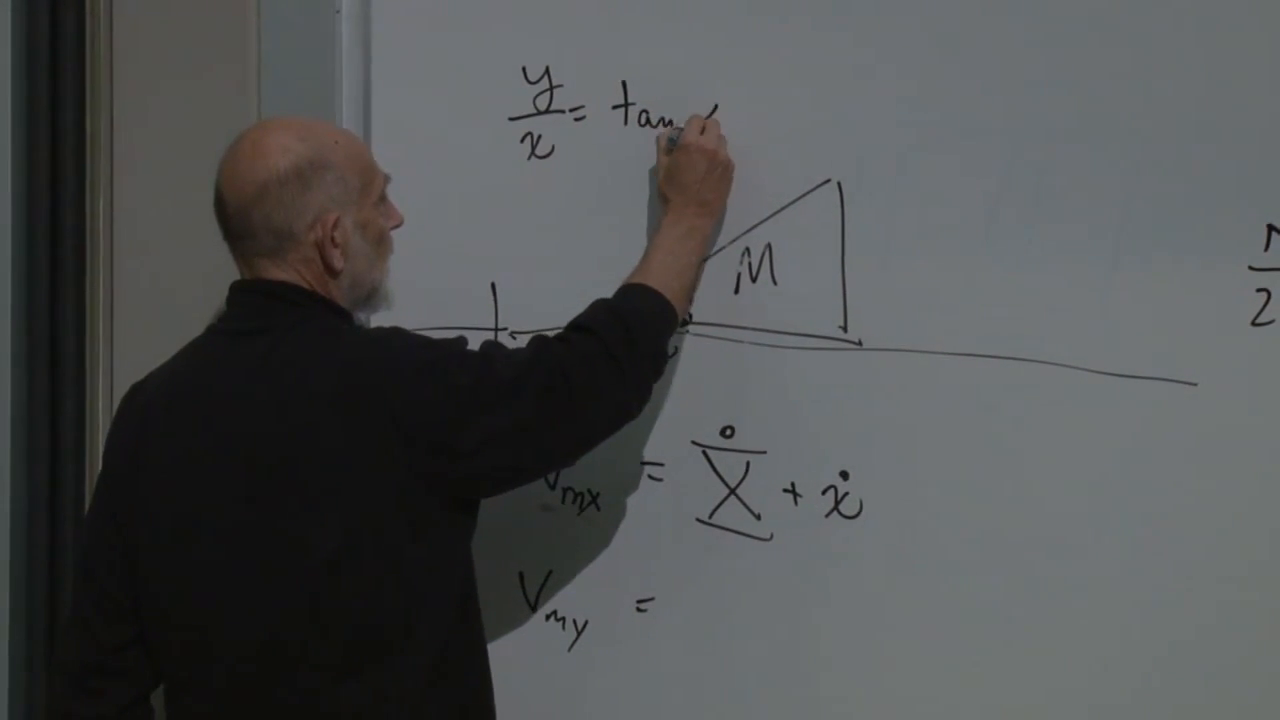
\includegraphics[width=0.84\textwidth]{lecture_06_figure_06.png}
  \caption{動くくさび、拘束された質点、および \(45^\circ\) の例で用いる水平・鉛直速度成分。}
  \lectureframe{00:10:25}
\end{figure}

くさびの運動エネルギーは
\begin{equation}
  T_{M}=\frac{M}{2}\dot X^2.
  \label{eq:l6-wedge-kinetic}
\end{equation}
である。質点の水平速度は \(\dot X+\dot x\) であり、その鉛直速度は \(\dot x\) である。したがってその運動エネルギーは
\begin{equation}
  T_m=\frac{m}{2}\left[(\dot X+\dot x)^2+\dot x^2\right].
  \label{eq:l6-particle-kinetic}
\end{equation}
となる。重力ポテンシャルの基準を \(x=0\) にとると、\(V=mgx\) である。ゆえに
\begin{equation}
  L=\frac{M}{2}\dot X^2
    +\frac{m}{2}\left[(\dot X+\dot x)^2+\dot x^2\right]
    -mgx.
  \label{eq:l6-wedge-lagrangian}
\end{equation}

\begin{figure}[htbp]
  \centering
  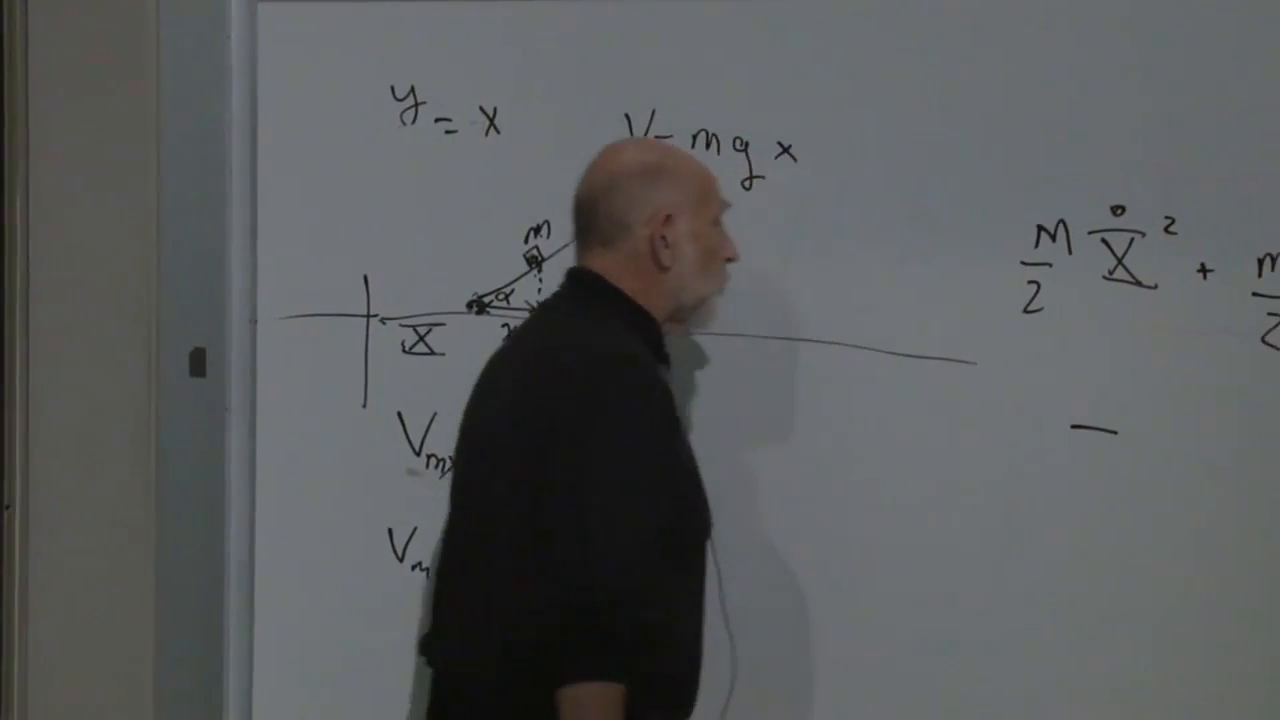
\includegraphics[width=0.86\textwidth]{lecture_06_figure_07.png}
  \caption{くさびの幾何、\(V=mgx\)、および二つの運動エネルギー寄与を黒板にまとめたもの。}
  \lectureframe{00:14:15}
\end{figure}

\subsection{正準運動量はラグランジアンによって定義される}

正準運動量は、単一の質点速度に基づく推測ではなく、ラグランジアンによって定義される。
\begin{align}
  p_X&=\frac{\partial L}{\partial\dot X}
      =M\dot X+m(\dot X+\dot x),
      \label{eq:l6-wedge-pX}\\
  p_x&=\frac{\partial L}{\partial\dot x}
      =m(\dot X+\dot x)+m\dot x.
      \label{eq:l6-wedge-px}
\end{align}
第一の表式は通常の全水平運動量である。くさびが \(M\dot X\) を寄与し、質点が
\(m(\dot X+\dot x)\) を寄与する。ここでは座標 \(X\) に共役な運動量として現れている。

\begin{figure}[htbp]
  \centering
  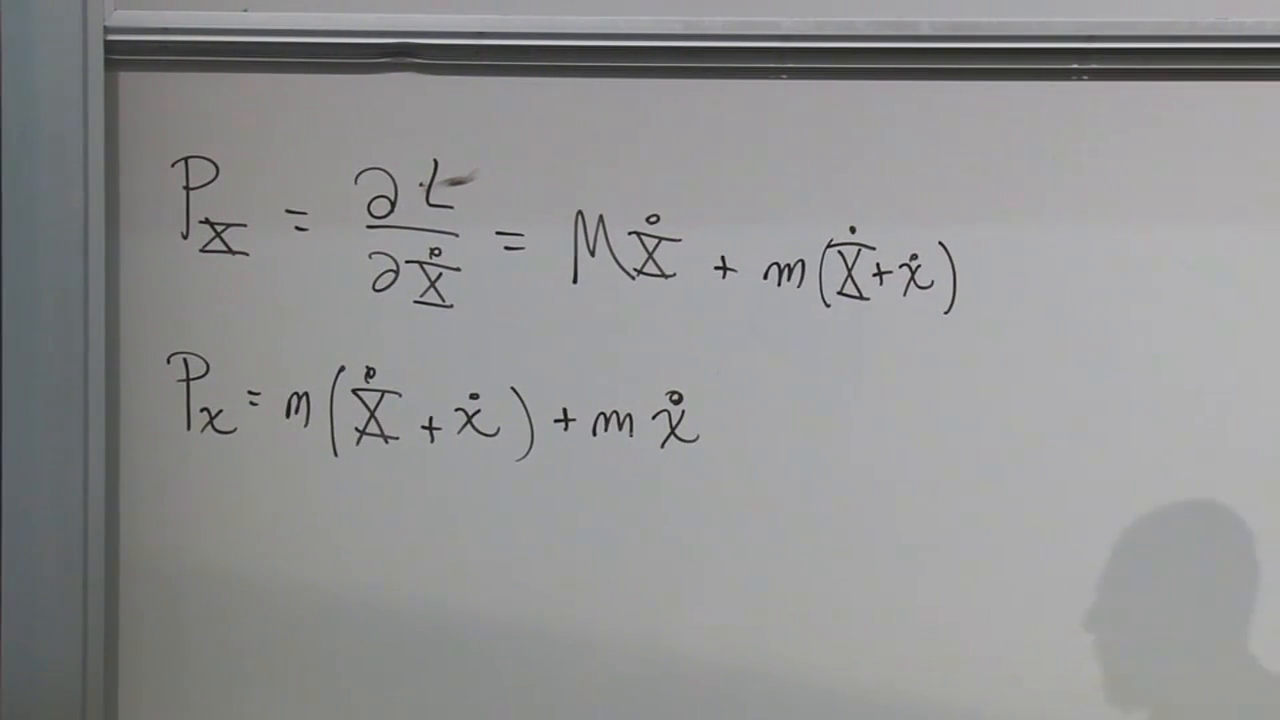
\includegraphics[width=0.86\textwidth]{lecture_06_figure_08.png}
  \caption{くさび座標 \(X\) および相対的な質点座標 \(x\) に共役な正準運動量。}
  \lectureframe{00:18:05}
\end{figure}

ラグランジアンは \(X\) に陽に依存しない。装置全体の水平並進は
\begin{equation}
  \delta X=\epsilon,
  \qquad
  \delta x=0.
  \label{eq:l6-wedge-translation}
\end{equation}
として作用する。したがって一般的な無限小対称性の規則
\begin{equation}
  \delta q_i=\epsilon f_i(q),
  \qquad
  Q=\sum_i p_i f_i
  \label{eq:l6-noether-rule}
\end{equation}
により \(Q=p_X\) が得られる。同値なことに、\(X\) は循環的であり、
\begin{equation}
  \dot p_X=\frac{\partial L}{\partial X}=0.
  \label{eq:l6-wedge-conservation}
\end{equation}

対応する鉛直並進対称性は存在しない。くさびは鉛直に動くことを許されておらず、質点の高さを変えると重力ポテンシャルが変化する。水平運動量は保存されるが、この拘束された部分系の鉛直運動量は保存されない。

相対座標について、Euler--Lagrange方程式は
\begin{equation}
  \dot p_x=\frac{\partial L}{\partial x}=-mg.
  \label{eq:l6-wedge-force}
\end{equation}
である。この行は黒板で符号の修正を要した。信頼できる道筋は\(L=T-V\)から始めることである。\(V=mgx\)であるから、Lagrangianの導関数は\(-mg\)となる。\(x\)が水平変位として導入されたという事実は、その方程式から重力を除かない。なぜなら、拘束条件がその水平変位を鉛直高さ\(y=x\)に結びつけているからである。

垂直抗力も反作用力も現れていない。そのような力は、拘束条件を維持するために必要とされる通りのものである。Newtonの方法ではそれらを導入し、加速度とともに解くことになるが、一般化座標はそれらを不要にした。

\section{二重振り子と座標の技法}

次に、単位長さの質量のない2本の棒から2つの単位質量を吊るす。第1の棒は下向きの鉛直線と角度\(\theta\)をなす。第2の自由度については選択肢がある。第2の絶対角\(\phi\)を用いることもできるし、棒の間の相対角\(\alpha\)を用いることもできる。

相対角の方がより本質を明らかにする選択である。一時的に重力を切る。装置全体の剛体回転は絶対的な向きを変えるが、棒の間の角度は変えない：
\begin{equation}
  \theta\longrightarrow\theta+\epsilon,
  \qquad
  \alpha\longrightarrow\alpha.
  \label{eq:l6-double-rotation}
\end{equation}
この選択では、回転対称性は1つの座標にのみ作用する。これは他の座標系が誤りであることを意味しない。対称性、したがって保存量をより見やすくするのである。

\begin{figure}[htbp]
  \centering
  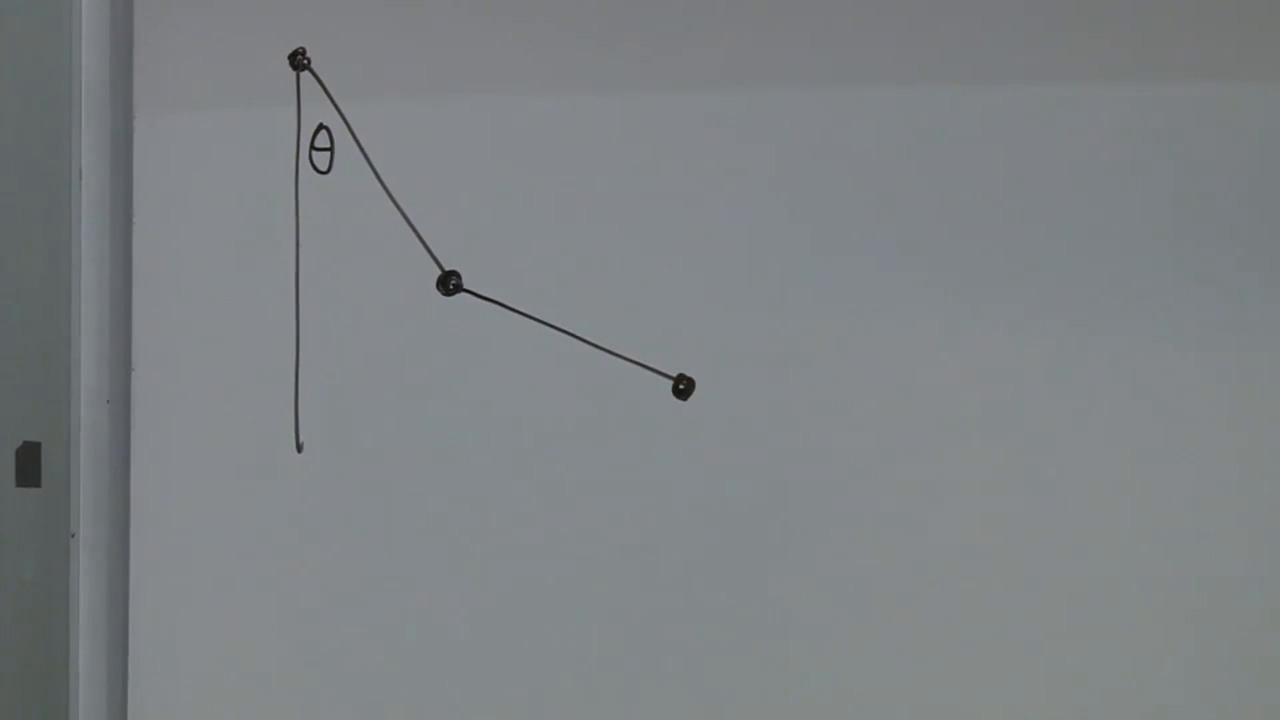
\includegraphics[width=0.76\textwidth]{lecture_06_figure_09.png}
  \caption{第1の絶対角を\(\theta\)、第1の棒に対する第2の棒の角度を\(\alpha\)とする二重振り子。}
  \lectureframe{00:29:20}
\end{figure}

運動エネルギーを得るには、一時的な記帳道具としてCartesian座標を用いる。鉛直座標を下向きに測ると、第1のおもりは
\begin{equation}
  x_1=\sin\theta,
  \qquad
  y_1=\cos\theta,
  \label{eq:l6-bob-one-position}
\end{equation}
にあり、したがって
\begin{equation}
  \dot x_1=\dot\theta\cos\theta,
  \qquad
  \dot y_1=-\dot\theta\sin\theta,
  \qquad
  \dot x_1^2+\dot y_1^2=\dot\theta^2.
  \label{eq:l6-bob-one-velocity}
\end{equation}
となる。第2のおもりは
\begin{align}
  x_2&=\sin\theta+\sin(\theta+\alpha),\\
  y_2&=\cos\theta+\cos(\theta+\alpha),
  \label{eq:l6-bob-two-position}
\end{align}
にあり、たとえば
\begin{equation}
  \dot x_2=\dot\theta\cos\theta
  +(\dot\theta+\dot\alpha)\cos(\theta+\alpha),
  \label{eq:l6-bob-two-xvelocity}
\end{equation}
であり、\(\dot y_2\)についても同様の式が成り立つ。

\begin{figure}[htbp]
  \centering
  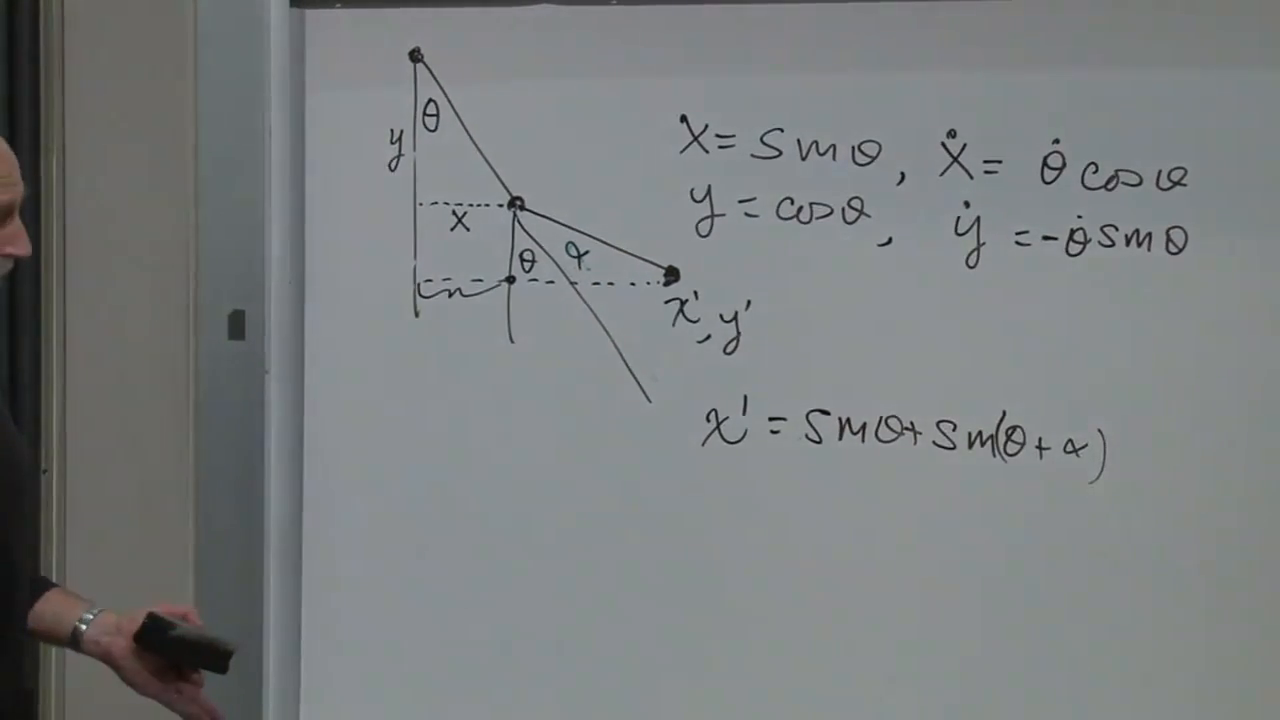
\includegraphics[width=0.88\textwidth]{lecture_06_figure_10.png}
  \caption{2つのおもりのための補助的なCartesian座標。これらは速度を計算するために用いられ、追加の自由度として導入されたものではない。}
  \lectureframe{00:35:25}
\end{figure}

2つの運動エネルギーを加えると、以下の整合した結果が得られる。交差項は
\begin{equation*}
  \cos A\cos B+\sin A\sin B=\cos(A-B).
\end{equation*}
から従う。
\begin{equation}
  T=\dot\theta^2
    +\frac12(\dot\theta+\dot\alpha)^2
    +\dot\theta(\dot\theta+\dot\alpha)\cos\alpha.
  \label{eq:l6-double-kinetic}
\end{equation}

\begin{classroomqa}
  \audiencequestion{この式はすでに両方のおもりの運動エネルギーを含んでいるのか、それとも1/2の因子が失われているのか。
  \lecturetimestamp{00:38:06--00:38:27}}
  \lecturerresponse{両方を含んでいる。それは
  \(\tfrac12(\dot x_1^2+\dot y_1^2+\dot x_2^2+\dot y_2^2)\)
から来る。2つの等しい寄与が合わさって第1項
  \(\dot\theta^2\)を生じるのであり、因子は失われていない。}
\end{classroomqa}

重力がなければ、\(L=T\)には\(\theta\)が陽に現れない。したがって
\begin{equation}
  \dot p_\theta=\frac{\partial L}{\partial\theta}=0,
  \label{eq:l6-double-angular-conservation}
\end{equation}
であり、\(p_\theta\)は全角運動量である。\(\theta\)が現れないという主張の正確な意味に注意せよ：\(\dot\theta\)は確かに現れるが、微分されていない座標は現れないのである。

重力を戻すと大域的回転対称性が破れる。上記の下向き鉛直の規約では、零点の1つの便利な選び方により
\begin{equation}
  V=-g(y_1+y_2)
   =-g\left[2\cos\theta+\cos(\theta+\alpha)\right].
  \label{eq:l6-double-potential}
\end{equation}
となる。付加定数は何も変えない。重要な点は、\(\theta\)が今や陽に現れるので、その共役運動量はもはや保存されないということである。Lagrangianが陽に時間に依存しないため、エネルギーは保存されたままである。

\begin{classroomqa}
  \audiencequestion{黒板の
  \(\dot\theta-\dot\alpha\)は
  \(\dot\theta+\dot\alpha\)であるべきか。
  \lecturetimestamp{00:43:00--00:43:54}}
  \lecturerresponse{ここで用いた向きでは正符号が必要である。それはEq.~\eqref{eq:l6-bob-two-position}の規約であり、Eq.~\eqref{eq:l6-double-kinetic}の運動エネルギーにも引き継がれている。正の\(\alpha\)の定義を逆にすれば対応する符号が変わるが、その場合すべての出現箇所を一貫して変えなければならない。黒板は2つの規約を混同していた。}
\end{classroomqa}

\begin{figure}[htbp]
  \centering
  \includegraphics[width=0.84\textwidth]{lecture_06_figure_02.png}
  \caption{重力なしの振り子の計算と
  \(\dot p_\theta=\partial L/\partial\theta\)。黒板の上の行は、質問で論じた符号の一貫しない局所的表記を保っている。正規化された式はEq.~\eqref{eq:l6-double-kinetic}である。}
  \lectureframe{00:45:50}
\end{figure}

\(T\)と\(V\)が分かれば、残りの方程式は微分によって得られる。棒の張力と固定長を強制する力は、再び座標の選択の中に消え去っている。

\subsection{保存則が意味することと意味しないこと}

\begin{classroomqa}
  \audiencequestion{二重振り子がカオス的であるかどうかを方程式から直接見ることができるか。
  \lecturetimestamp{00:44:57--00:45:25}}
  \lecturerresponse{通常は単純な目視ではできない。パラメータやエネルギーが変化するにつれて、系は規則的挙動からカオス的挙動へ移行しうる。この主題には、方程式の見かけ以上の構造が必要であり、後で取り上げる。}
\end{classroomqa}

\begin{classroomqa}
  \audiencequestion{保存系では、すべての\(\dot p_i\)が
  ゼロに等しいか。
  \lecturetimestamp{00:45:25--00:46:24}}
  \lecturerresponse{いいえ。一般式は
  \(\dot p_i=\partial L/\partial q_i\)である。これが消えるのは\(q_i\)が
  循環的である場合に限る。循環座標とは、対称性によって一方の座標を
  他方の座標を固定したまま移すことができた、特に単純な場合である。}
\end{classroomqa}

目的が数値的な時間発展だけであるなら、不便な座標系でも機能する。単に方程式が長くなるだけである。巧妙な座標系を選ぶことの報酬は概念的である。すなわち、方程式を解く前に保存運動量が見えることである。

\begin{classroomqa}
  \audiencequestion{重力がなければ、二重振り子は単一の自由振り子と同じように
  単純に振る舞うか。
  \lecturetimestamp{00:47:02--00:47:35}}
  \lecturerresponse{単一の自由回転子は、その一つの角運動量が運動を定めるため、
  一様に回転する。二重振り子は、全角運動量を保存しながら、非常に
  複雑な相対運動を行い得る。両方の角速度が初期にゼロであれば静止したままであり、
  そうでなければ二つの部分が相互作用する。}
\end{classroomqa}

\begin{classroomqa}
  \audiencequestion{重力が存在しないとき、\(\dot\theta\)と\(\dot\alpha\)は
  それぞれ一定か。
  \lecturetimestamp{00:47:36--00:52:42}}
  \lecturerresponse{いいえ。保存則が言うのは\(\dot p_\theta=0\)であり、
  \(\ddot\theta=0\)や\(\ddot\alpha=0\)ではない。\(p_\theta=\partial L/\partial\dot\theta\)の表式には
  両方の角速度が含まれ、\(\alpha\)に依存する。棒はトルクを伝え、
  二つのおもりが角運動量とエネルギーを交換することを可能にする。これは
  ばねで結ばれた二つの質量に類似している。全運動量と重心速度は一定であるが、
  個々の速度は振動する。回転の場合の類似物は特定の集団的な組み合わせであり、
  どちらか一方の角度そのものではない。}
\end{classroomqa}

\begin{classroomqa}
  \audiencequestion{角運動量を交換する力は
  棒を通して伝わるのか。
  \lecturetimestamp{00:52:43--00:53:34}}
  \lecturerresponse{はい。棒に沿って伝わる力は、他方の運動の支点を
  通る必要はないので、トルクを及ぼし得る。トルクとは単に力の回転的な傾向であり、
  ここではそれがゼロでない個々の角加速度を生じさせる。}
\end{classroomqa}

\section{第三の定式化としてのハミルトニアン}

ハミルトニアンはエネルギーであるが、それはその第一の意義にすぎない。それは
力学の第三の定式化の基礎でもある。ニュートンの方程式は
力と加速度を用いる。停留作用の原理は
オイラー--ラグランジュ方程式を与える。ハミルトン力学は正則系に対して後者と
等価であるが、その変数と幾何学は異なって見える。

\(q_i\)と\(\dot q_i\)の代わりに、\(q_i\)とその共役運動量
\(p_i\)を用いる。\(n\)個の自由度をもつ系の状態は、どちらの記述でも\(2n\)
個の数を必要とする。すなわち位置と速度、または位置と
運動量である。両者をつなぐ橋は
\begin{equation}
  p_i=\frac{\partial L}{\partial\dot q_i}.
  \label{eq:l6-legendre-map}
\end{equation}
である。これらの関係を速度\(\dot q_i(q,p)\)について逆に解けるとき、
\begin{equation}
  H(q,p)=\sum_i p_i\dot q_i-L(q,\dot q).
  \label{eq:l6-hamiltonian-definition}
\end{equation}
と定義する。右辺の速度はその後、\(q\)と\(p\)を用いて消去される。
この可逆性が正則ルジャンドル変換の仮定である。特異な
ラグランジアンはより一般的な拘束の理論を必要とし、この初等的な構成では
扱われない。

\subsection{微積分以前の可逆性}

矢印で結ばれた抽象状態の有限集合を思い出そう。決定論的な規則であっても、
二つの以前の状態が一つの後の状態へ流れ込むならば、可逆でないことがある。
未来は一意であるが、過去はそうではない。すべての矢印を逆にすると、
反対の欠陥が生じる。すなわち一つの状態が複数の未来へ分岐する。
第一の図では矢印は収束し、第二の図では発散する。

\begin{figure}[htbp]
  \centering
  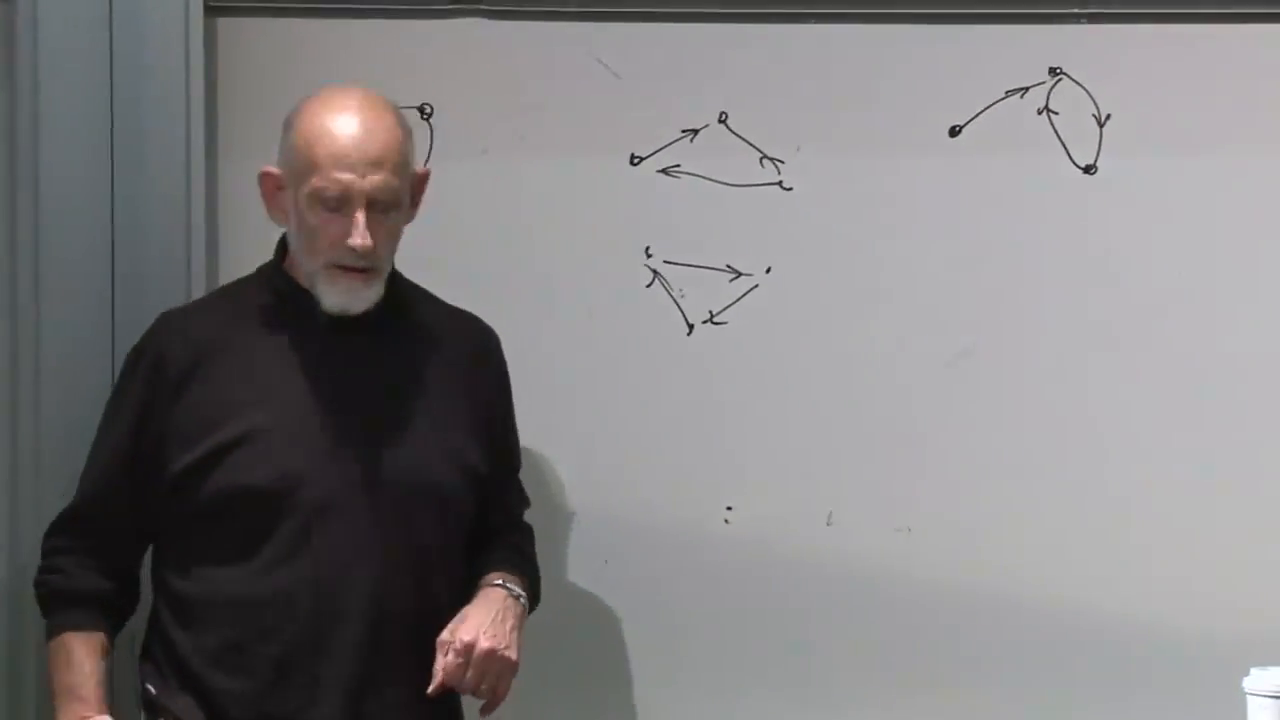
\includegraphics[width=0.86\textwidth]{lecture_06_figure_11.png}
  \caption{可逆な循環と、禁じられた収束および発散を対比するために用いられる
  抽象状態写像。}
  \lectureframe{00:56:20}
\end{figure}

ハミルトン流がこの命題の連続版を与えることになる。相空間の点の雲は
移動し変形し得るが、状態間の区別を破壊する吸い込みや、一つの状態から
複数の未来を生み出す源を得ることはできない。証明は後回しにする。今は図が
幾何学の動機を与える。

\begin{classroomqa}
  \audiencequestion{抽象状態図は重力場中を運動する物体として
  解釈されるべきか。
  \lecturetimestamp{00:58:02--00:58:35}}
  \lecturerresponse{いいえ。点は単に抽象状態であり、矢印は状態を変える
  規則を指定する。この図には空間的または重力的な意味は
  何も割り当てられていない。}
\end{classroomqa}

\begin{classroomqa}
  \audiencequestion{禁止された収束状態写像は、ブラックホールとどのように区別されるのか。
  \lecturetimestamp{00:58:40--00:59:28}}
  \lecturerresponse{困難と微妙さを伴ってのみ区別される。これはもっともな問いであるが、正しい答えには完全な状態とその量子重力論的発展についての注意深い記述が必要である。初等的な図だけではこれを決着させるのに十分ではない。}
\end{classroomqa}

\section{位相空間に適合させた振動子}

一般方程式を導出する前に、意図的に適合させた変数で書かれた調和振動子を考える：
\begin{equation}
  L=\frac{1}{2\omega}\dot q^2-\frac{\omega}{2}q^2.
  \label{eq:l6-rescaled-lagrangian}
\end{equation}
その共役運動量は
\begin{equation}
  p=\frac{\partial L}{\partial\dot q}=\frac{\dot q}{\omega},
  \qquad
  \dot q=\omega p.
  \label{eq:l6-rescaled-momentum}
\end{equation}
式~\eqref{eq:l6-hamiltonian-definition}に代入すると
\begin{align}
  H&=p\dot q-L\\
   &=\omega p^2-\frac{\omega p^2}{2}+\frac{\omega q^2}{2}
    =\frac{\omega}{2}(p^2+q^2).
  \label{eq:l6-oscillator-hamiltonian}
\end{align}

\begin{figure}[htbp]
  \centering
  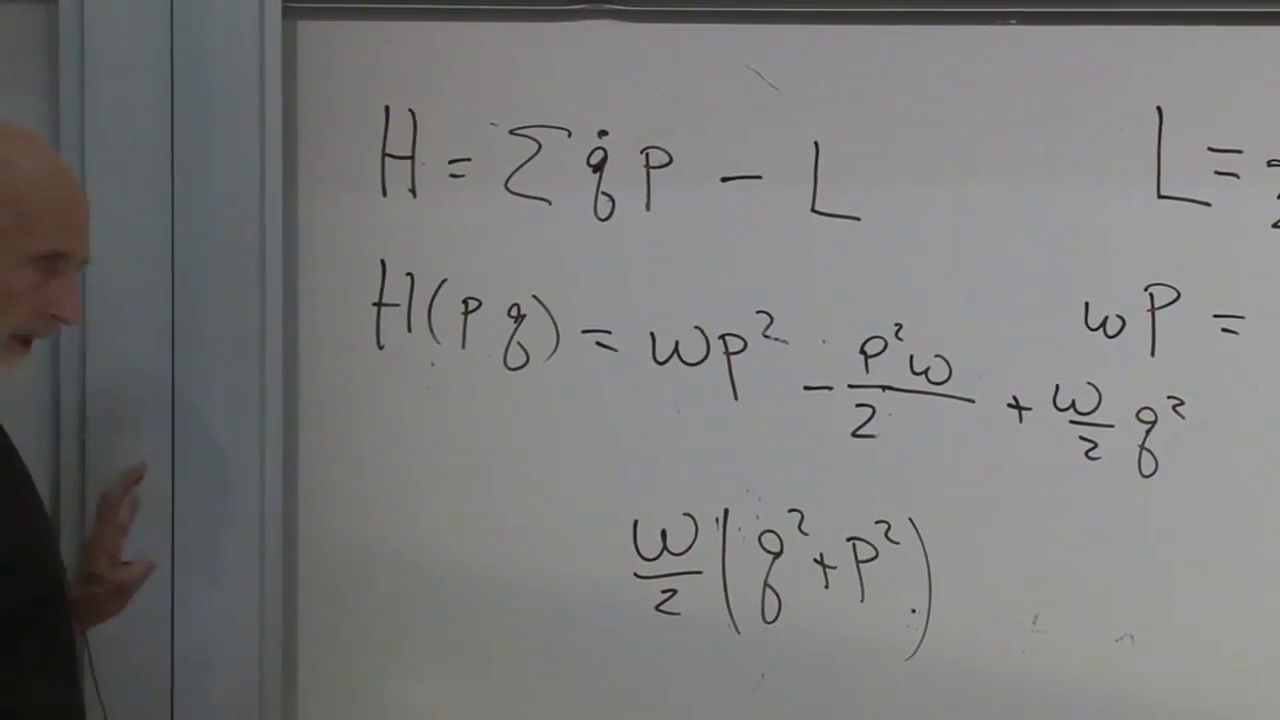
\includegraphics[width=0.86\textwidth]{lecture_06_figure_12.png}
  \caption{適合させた振動子のルジャンドル変換と対称なハミルトニアン\(H=\tfrac{\omega}{2}(p^2+q^2)\)。}
  \lectureframe{01:08:20}
\end{figure}

\(q\)と\(p\)の空間が位相空間である。1自由度では2次元平面が得られ、2自由度では4次元位相空間が得られる。振動子のエネルギーを固定すると、
\begin{equation}
  p^2+q^2=\frac{2H}{\omega},
  \label{eq:l6-energy-circle}
\end{equation}
したがって軌道は円上にとどまる。エネルギー保存により、運動はそのような曲線の一つに閉じ込められる。

\begin{figure}[htbp]
  \centering
  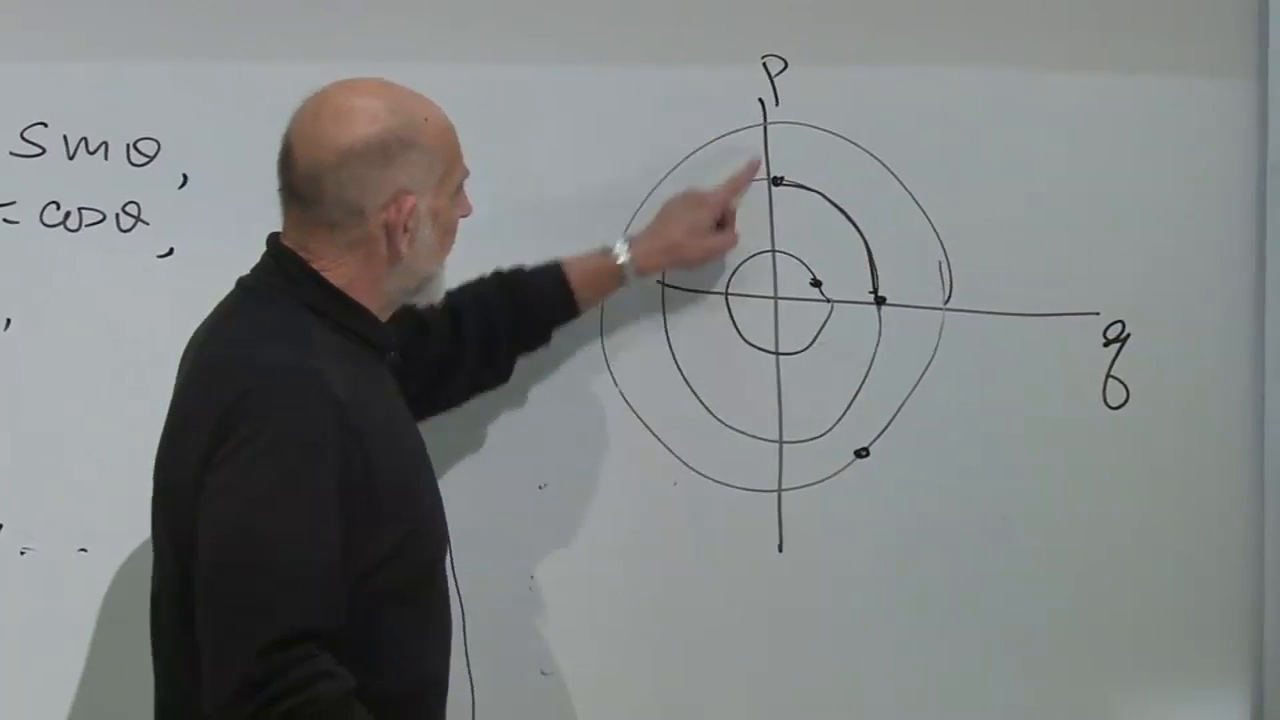
\includegraphics[width=0.82\textwidth]{lecture_06_figure_13.png}
  \caption{振動子の位相平面における入れ子状の等エネルギー円。\(q\)が水平方向、\(p\)が垂直方向である。}
  \lectureframe{01:13:20}
\end{figure}

\section{ハミルトンの方程式の導出}

この導出は多変数関数の微分に関する演習である。\(F(q,p)\)に対して、
\begin{equation}
  \delta F=\sum_i\left(
  \frac{\partial F}{\partial q_i}\delta q_i
  +\frac{\partial F}{\partial p_i}\delta p_i\right).
  \label{eq:l6-total-differential}
\end{equation}
係数はどちらの方向にも読める。\(\delta q_i\)の係数は\(\partial F/\partial q_i\)であり、\(\delta p_i\)の係数は\(\partial F/\partial p_i\)である。

次に\(H\)を定義する式を変分する：
\begin{align}
  \delta H
  &=\sum_i\left(\dot q_i\,\delta p_i
       +p_i\,\delta\dot q_i\right)-\delta L\\
  &=\sum_i\left(\dot q_i\,\delta p_i
       +p_i\,\delta\dot q_i
       -\frac{\partial L}{\partial q_i}\delta q_i
       -\frac{\partial L}{\partial\dot q_i}\delta\dot q_i\right).
  \label{eq:l6-vary-hamiltonian}
\end{align}
\(\partial L/\partial\dot q_i=p_i\)であるから、二つの\(\delta\dot q_i\)の項は相殺する。オイラー--ラグランジュ方程式により\(\partial L/\partial q_i=\dot p_i\)となり、
\begin{equation}
  \delta H=\sum_i\left(\dot q_i\,\delta p_i
                     -\dot p_i\,\delta q_i\right).
  \label{eq:l6-reduced-variation}
\end{equation}が残る。

\begin{figure}[htbp]
  \centering
  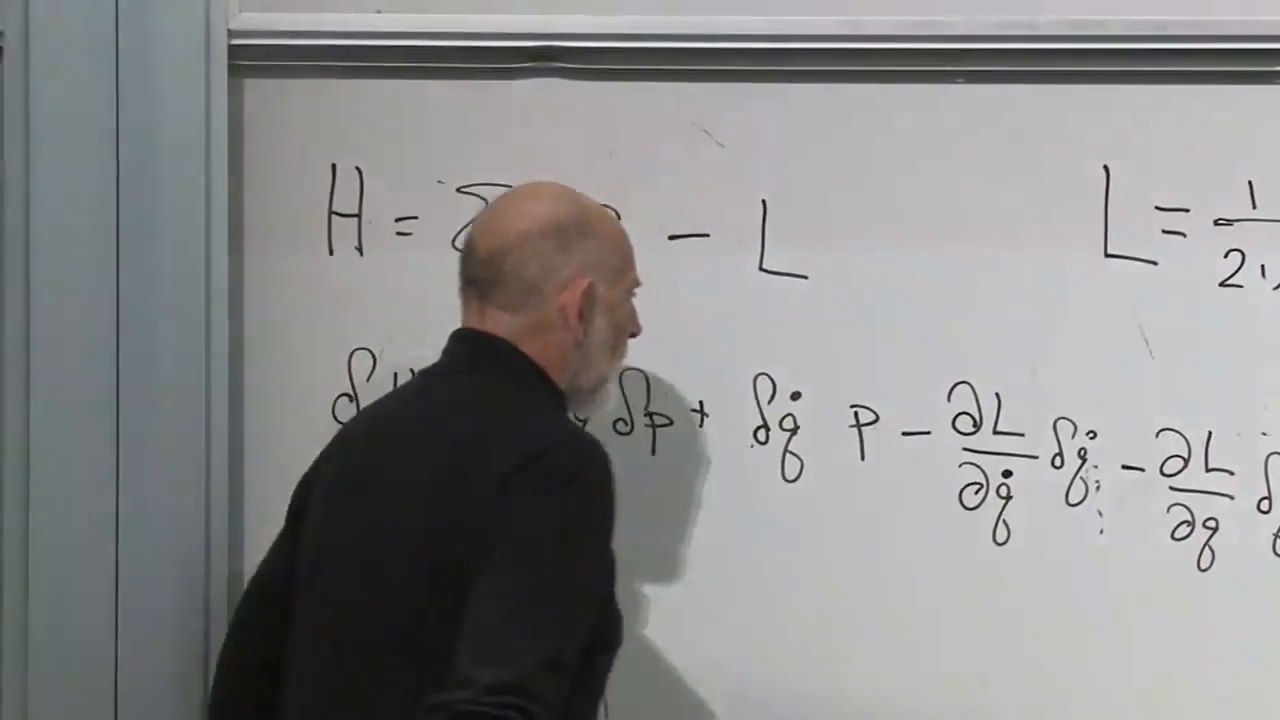
\includegraphics[width=0.86\textwidth]{lecture_06_figure_14.png}
  \caption{\(p_i\,\delta\dot q_i\)の項が相殺する前の\(\delta H\)の積の法則による展開。}
  \lectureframe{01:18:40}
\end{figure}

式~\eqref{eq:l6-reduced-variation}を式~\eqref{eq:l6-total-differential}の一般微分と比較すると、独立な係数からハミルトンの方程式が得られる：
\begin{equation}
  \boxed{
  \dot q_i=\frac{\partial H}{\partial p_i},
  \qquad
  \dot p_i=-\frac{\partial H}{\partial q_i}.}
  \label{eq:l6-hamilton-equations}
\end{equation}

\begin{figure}[htbp]
  \centering
  \includegraphics[width=0.78\textwidth]{lecture_06_figure_03.png}
  \caption{ハミルトニアンの定義、その変分、および枠で囲まれた正準方程式。}
  \lectureframe{01:22:18}
\end{figure}

\(n\)個の座標に対して、これらは\(2n\)個の一階方程式である。一方、オイラー--ラグランジュ形式は\(n\)個の二階方程式を与える。初期データの量と物理的内容は同一である。

\section{剛体回転としての振動子の運動}

式~\eqref{eq:l6-hamilton-equations}を式~\eqref{eq:l6-oscillator-hamiltonian}に適用すると
\begin{equation}
  \dot q=\omega p,
  \qquad
  \dot p=-\omega q.
  \label{eq:l6-oscillator-first-order}
\end{equation}
が得られる。第一の方程式を微分し、第二の方程式を用いると、
\begin{equation}
  \ddot q=\omega\dot p=-\omega^2q.
  \label{eq:l6-oscillator-second-order}
\end{equation}
したがって、二つの一階方程式は、運動量の定義とともに、まさに通常の二階の振動子方程式である。

位相空間において、\((q,p)\)における速度ベクトルは\((\dot q,\dot p)=(\omega p,-\omega q)\)であり、エネルギー円に接している。すべての半径は同じ角速度\(\omega\)で回転する。平面全体は剛体の風車、あるいは非圧縮の仮想流体として想像してよい。その点は循環するが、吸い込み口に押し込まれたり、湧き出し口から飛び散ったりはしない。

\begin{figure}[htbp]
  \centering
  \includegraphics[width=0.86\textwidth]{lecture_06_figure_04.png}
  \caption{入れ子状の位相空間軌道に分布する初期点の雲。ハミルトン的発展は、雲を好ましい状態へと崩壊させるのではなく、動かす。}
  \lectureframe{01:39:27}
\end{figure}

\begin{figure}[htbp]
  \centering
  \includegraphics[width=0.90\textwidth]{lecture_06_figure_05.png}
  \caption{振動子の位相肖像と、それに相当するオイラー--ラグランジュ方程式\(\ddot q/\omega=-\omega q\)。}
  \lectureframe{01:42:10}
\end{figure}

次の段階は、流体の類推を定理に変えることである。ハミルトン的流れには局所的な収束も発散もない。この結果は、連続力学を、講義の冒頭で考察した可逆な状態写像と再び結びつける。

\section{座標の選択を露わにする問い}

\begin{classroomqa}
  \audiencequestion{速度が\(q\)と\(p\)で解けるという仮定は、定理なのか、それとも物理系の経験的性質なのか。
  \lecturetimestamp{01:29:08--01:29:45}}
  \lecturerresponse{この初等的な展開の範囲内では、それは経験的な規則性であり、量子力学からのより深い動機づけがある。より正確には、式~\eqref{eq:l6-legendre-map}は速度に関する非特異なヤコビアンを持たなければならない。現代の力学には、特に拘束系やゲージ系において、重要な特異ラグランジアンも含まれるが、それらのハミルトン形式には追加の拘束機構が必要である。}
\end{classroomqa}

単位に関する異議は、なぜ振動子が式~\eqref{eq:l6-rescaled-lagrangian}という見慣れない形で書かれたのかを説明する。代わりに通常の座標\(x\)から始めよう：
\begin{equation}
  L=\frac{m}{2}\dot x^2-\frac{k}{2}x^2,
  \qquad
  \omega=\sqrt{\frac{k}{m}}.
  \label{eq:l6-ordinary-oscillator}
\end{equation}
次を選ぶ：
\begin{equation}
  q=(km)^{1/4}x.
  \label{eq:l6-oscillator-rescaling}
\end{equation}
すると\(q^2=\sqrt{km}\,x^2\)および\(\dot q^2=\sqrt{km}\,\dot x^2\)となり、これにより式~\eqref{eq:l6-ordinary-oscillator}は正確に式~\eqref{eq:l6-rescaled-lagrangian}へと変換される。新しい\(q\)は適合させた一般化座標であって長さではなく、その共役な\(p\)は通常の力学的運動量\(p_x=m\dot x\)ではない。

\begin{figure}[htbp]
  \centering
  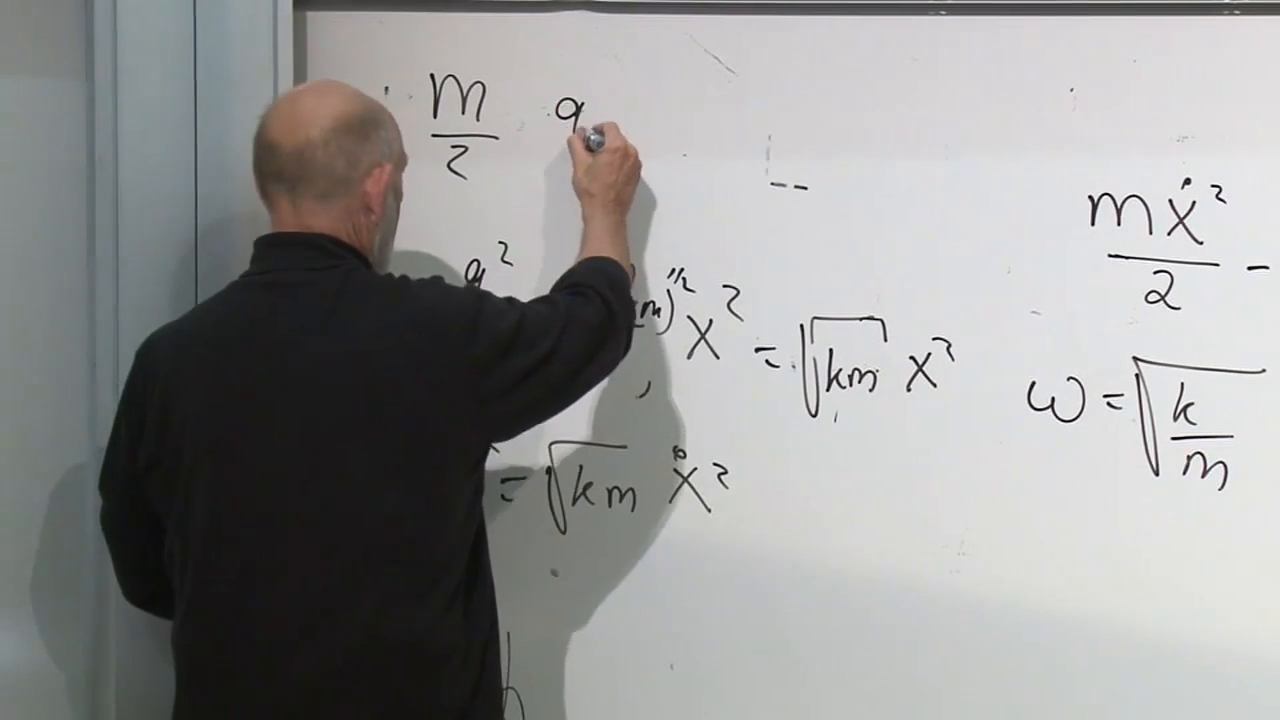
\includegraphics[width=0.86\textwidth]{lecture_06_figure_15.png}
  \caption{通常の振動子座標\(x\)から適合座標\(q=(km)^{1/4}x\)への次元的な再スケーリング。}
  \lectureframe{01:36:10}
\end{figure}

\begin{classroomqa}
  \audiencequestion{\(\omega p=\dot q\)はどのようにして次元的に整合し得るのか、そしてなぜこれらの変数が選ばれたのか。
  \lecturetimestamp{01:29:46--01:39:22}}
  \lecturerresponse{記号\(q\)は長さの次元を持つ必要はなく、その共役な\(p\)は\(m\dot x\)の次元を持つ必要もない。式~\eqref{eq:l6-oscillator-rescaling}の再スケーリングはラグランジアンの次元を保ち、\(q\)と\(p\)が\(H\)に左右対称に入るようにする。元の変数では
  \[
    H=\frac{p_x^2}{2m}+\frac{kx^2}{2},
  \]
  であるから、\((x,p_x)\)平面における等エネルギー曲線は楕円である。適合させた\((q,p)\)平面ではそれらは円である。この再スケーリングはその対称性を可視化するために選ばれた。}
\end{classroomqa}

\begin{classroomqa}
  \audiencequestion{\(2n\)個の一階ハミルトン方程式が、どのようにして\(n\)個の二階ラグランジュ方程式と等価になり得るのか。
  \lecturetimestamp{01:39:24--01:42:30}}
  \lecturerresponse{振動子の場合、\(\dot q=\omega p\)を微分し\(\dot p=-\omega q\)を代入すると、その組は\(\ddot q=-\omega^2q\)となる。ラグランジアンから直接始めると
  \[
    \frac{d}{dt}\left(\frac{\dot q}{\omega}\right)
      =-\omega q,
  \]
  が得られ、これは同じ二階方程式である。一方のハミルトン方程式は速度から運動量を定義するものと見なすことができ、他方はその運動量を時間発展させる。}
\end{classroomqa}

\section{なぜ位相空間とポテンシャルエネルギーが重要か}

\begin{classroomqa}
  \audiencequestion{ハミルトニアンの威力は、位相空間が配位空間よりも優れた幾何学的表現であることを意味するのか。
  \lecturetimestamp{01:42:33--01:44:38}}
  \lecturerresponse{それらは異なる目的を果たす。位相空間は、周期、等エネルギー面、そして収束や発散の不在をきわめて透明にする。配位空間は他の問いにはより適しているかもしれない。\(H\)を強調するより深い理由は、それが量子力学において中心的でより直観的な対象となり、この力学が向かう現代の主題の一つとなるからである。}
\end{classroomqa}

\begin{classroomqa}
  \audiencequestion{ポテンシャルエネルギーは力の積分と見なすべきか。
  \lecturetimestamp{01:44:40--01:45:45}}
  \lecturerresponse{保存力に対しては、その記述は定数分の不定性と適切な符号を除いて妥当である。より有用な方向は、ポテンシャルを第一義的なものと見なし、そこから一般化力を導くことである：
  \[
    F_i=-\frac{\partial V}{\partial q_i}.
  \]
  これはまさに、\(L=T-V\)で\(\dot p_i=\partial L/\partial q_i\)に現れる項であり、運動エネルギーが\(q_i\)に陽に依存しない場合のものである。}
\end{classroomqa}

\begin{classroomqa}
  \audiencequestion{現代物理学へのこの道は、どのようなフロンティア問題を照らし出すことを意図しているのか。
  \lecturetimestamp{01:45:46--01:47:47}}
  \lecturerresponse{この道は量子重力と宇宙論へと導く；ヒッグスセクターとニュートリノを含む素粒子物理学；相対性理論；弦理論；そして量子場の理論である。永続する理論的問題は、これらの断片を一つの首尾一貫した構造に収めること、特に量子力学と重力、そして宇宙論と素粒子物理学を両立させることである。これは2011年に現れたフロンティアの記述であり、その解決がすでに知られていたという主張ではない。}
\end{classroomqa}

二つの拘束された例と振動子は、今や一つの描像に収まる。一般化座標は不要な力を取り除く。対称性は保存する正準運動量を選び出す。ルジャンドル変換は速度を運動量に置き換え、ハミルトンの方程式は力学を位相空間上の流れへと変える。振動子にとってその流れは剛体回転であり、一般の系ではその幾何学が可逆運動の正確で連続的な意味を与えるであろう。